\documentclass[12pt, letterpaper]{../assignment}
\usepackage{graphicx}
\usepackage{courier}
\usepackage{minted}
\usepackage{amsmath}
\usepackage{commath}
\usepackage{amssymb}
\usepackage{amsfonts} 
\usepackage{cancel}


\usemintedstyle{monokai}
\oddsidemargin = 0pt
\exercisesheet{Module 3}{Practice Assignment}
\student{Austin Barrilleaux}
\courselabel{EN 525.609}
\semester{Fall 2023}
\usepackage[backend=bibtex,style=numeric,sorting=none]{biblatex}
\bibliography{reference}
\usepackage{color}
\definecolor{light-gray}{rgb}{0.2,0.2,0.2}
\setminted{bgcolor=light-gray}
\setlength{\parindent}{0pt}

\makeatletter
\patchcmd{\minted@colorbg}{\noindent}{\medskip\noindent}{}{}
\apptocmd{\endminted@colorbg}{\par\medskip}{}{}
\makeatother

\begin{document}
\subsection*{Problem 1}
\subsubsection*{Solve the following practice problems in the 9th edition textbook.\\
\begin{itemize}
    \item Chapter 3:
    \begin{itemize}
        \item 10-1 (c) (use MATLAB if / as needed)
    \end{itemize}
\end{itemize}}

\subsubsection*{The following differential equation represents a linear time-invariant system.
Write the following dynamic equation (state equations and output equations) in vector-matrix form:\\
{\boldmath $$ \frac{d^3 y(t)}{d t^3} + 5 \frac{d^2 y(t)}{d t^2} + 3\frac{d y(t)}{d t} + y(t) + \int_{0}^{t} y(\tau) d \tau = r(\tau) $$}}

We can establish the following relationships:

\begin{equation*}
    \begin{aligned}
        x_1(t) = &\int_{0}^{t} y(\tau) d \tau\\
        x_2(t) = &\dot{x}_1 = y(t)\\
        x_3(t) = &\dot{x}_2 = \frac{d y(t)}{d t}\\
        x_4(t) = &\dot{x}_3 = \frac{d^2 y(t)}{d t^2}\\
        &\dot{x}_4 = \frac{d^3 y(t)}{d t^3}
    \end{aligned}
\end{equation*}

We can rewrite the dynamic equation in question as:

$$ \frac{d^3 y(t)}{d t^3} = - 5 \frac{d^2 y(t)}{d t^2} - 3\frac{d y(t)}{d t} - y(t) - \int_{0}^{t} y(\tau) d \tau + r(\tau) $$

The standard matrix state equations are:

\begin{equation*}
    \begin{aligned}
        \dot{x}(t) &= A x(t) + B u(t)\\
        y(t) &= C x (t) + D u(t)
    \end{aligned}
\end{equation*}


Given the above relationships, we can write the dynamic equation as components of the standard matrix equations in the following matrix form:

\begin{equation*}
    A = \begin{bmatrix}
        0 & 1 & 0 & 0 \\
        0 & 0 & 1 & 0 \\
        0 & 0 & 0 & 1 \\
        -1 & -1 & -3 & -5
    \end{bmatrix}
\end{equation*}

\begin{equation*}
    B = \begin{bmatrix}
        0\\ 0\\ 0\\ 1
    \end{bmatrix}
\end{equation*}

\begin{equation*}
    C = \begin{bmatrix}
        0 & 1 & 0 & 0
    \end{bmatrix}
\end{equation*}

Therefore, the state equation is:

\begin{answer}
    \begin{equation*}
        \begin{bmatrix}
            \dot{x}_1\\ \dot{x}_2\\ \dot{x}_3\\ \dot{x}_4
        \end{bmatrix}=
        \begin{bmatrix}
            0 & 1 & 0 & 0 \\
            0 & 0 & 1 & 0 \\
            0 & 0 & 0 & 1 \\
            -1 & -1 & -3 & -5
        \end{bmatrix}
        \begin{bmatrix}
            x_1\\ x_2\\ x_3\\ x_3
        \end{bmatrix}
        + \begin{bmatrix}
            0\\ 0\\ 0\\ 1
        \end{bmatrix} r(\tau)
    \end{equation*}
\end{answer}

And the output equation is:

\begin{answer}
    \begin{equation*}
        y(t)=
        \begin{bmatrix}
            0 & 1 & 0 & 0
        \end{bmatrix}
        \begin{bmatrix}
            x_1\\ x_2\\ x_3\\ x_3
        \end{bmatrix}
    \end{equation*}
\end{answer}


\subsection*{Problem 1}
\subsubsection*{Consider the block diagram of the following feedback control system:}


\begin{figure}[H]
    \centering
    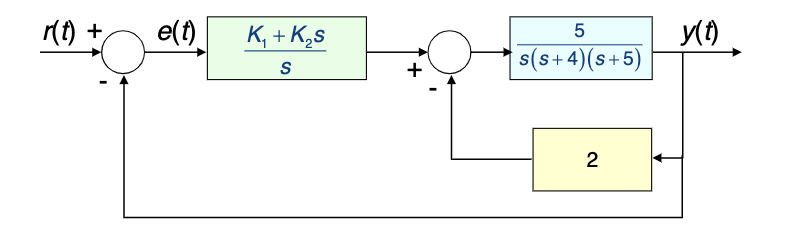
\includegraphics[scale=1]{figures/problem2.png}
    \caption{Problem 2}
    \label{Fig:prob2}
\end{figure}

\subsubsection*{(a) Find the open-loop TF Y(s) / E(s) and the closed-loop TF Y(s) / R(s)}

The open loop transfer function is simply the multiplication of the green and blue blocks:

$$ \frac{Y(s)}{E(s)} = \left(\frac{K_1 + K_2 s}{s}\right) \left(\frac{5}{s(s+4)(s+5)}\right) $$

Or
\begin{answer}
    $$ \frac{Y(s)}{E(s)} = \frac{5(K_1 + K_2 s)}{s^2(s+4)(s+5)} $$
\end{answer}

The to solve for the closed loop transfer function, first we reduce the blue and yellow blocks.
They reduce to:

\begin{equation*}
    \frac{\frac{5}{s(s+4)(s+5)}}{1 + 2\frac{5}{s(s+4)(s+5)}} = 
    \frac{5}{s(s+4)(s+5) + 10}
\end{equation*}

This combines with the green block to get:

\begin{equation*}
    \frac{5(K_1 + K_2 s)}{s^2(s+4)(s+5) + 10s}
\end{equation*}

Which is the last block in a unity feedback loop, giving us the final transfer function of 

$$ \frac{Y(s)}{R(s)} = \frac{\frac{5(K_1 + K_2 s)}{s^2(s+4)(s+5) + 10s}}{1 +\frac{5(K_1 + K_2 s)}{s^2(s+4)(s+5) + 10s}}
= \frac{5(K_1 + K_2 s)}{s^2(s+4)(s+5) + 10s +5(K_1 + K_2 s)} $$

The closed loop transfer function is:

\begin{answer}
$$ \frac{Y(s)}{R(s)} = \frac{5(K_1 + K_2 s)}{s^2(s+4)(s+5) + 10s +5(K_1 + K_2 s)} $$
\end{answer}

\subsubsection*{(b) Write the dynamic equations in the form:\\
{\boldmath} \begin{equation*}
    \begin{aligned}
        \dot{\bar{x}}(t) &= A \bar{x}(t) + B \bar{u}(t)\\
        y(t) &= C \bar{x} (t) + D \bar{u}(t)
    \end{aligned}
\end{equation*}}

To do this for the open loop case, we must first expand the numerator and the denominator to get:

$$ \frac{Y(s)}{E(s)} = \frac{5K_1 + 5K_2 s}{s^4 + 9 s^3 + 20 s^2} $$

Then separate the equation into the form:

$$ \frac{Y(s)}{E(s)} = \frac{Y(s)}{V(s)} \frac{V(s)}{E(s)} = \left(\frac{5K_1 + 5K_2 s}{1}\right) \left(\frac{1}{s^4 + 9 s^3 + 20 s^2}\right) $$

We can put this into the state space form:

\begin{answer}
    \begin{equation*}
        \begin{bmatrix}
            \dot{x}_1\\ \dot{x}_2\\ \dot{x}_3\\ \dot{x}_4
        \end{bmatrix}=
        \begin{bmatrix}
            0 & 1 & 0 & 0 \\
            0 & 0 & 1 & 0 \\
            0 & 0 & 0 & 1 \\
            0 & 0 & -20 & -9
        \end{bmatrix}
        \begin{bmatrix}
            x_1\\ x_2\\ x_3\\ x_4
        \end{bmatrix}
        + \begin{bmatrix}
            0\\ 0\\ 0\\ 1
        \end{bmatrix} r(t)
    \end{equation*}
\end{answer}
\begin{answer}
    \begin{equation*}
        y(t)=
        \begin{bmatrix}
            5 K_1 & 5 K_2 & 0 & 0
        \end{bmatrix}
        \begin{bmatrix}
            x_1\\ x_2\\ x_3\\ x_4
        \end{bmatrix}
    \end{equation*}
\end{answer}

To do this for the closed loop case, we must first expand the numerator and the denominator to get:

$$ \frac{Y(s)}{R(s)} = \frac{5 K_1 + 5 K_2 s}{s^4 + 9 s^3 + 20 s^2 + (5 K_2 + 10) s + 5 K_1} $$

Then separate the equation into the form:

$$ \frac{Y(s)}{E(s)} = \frac{Y(s)}{V(s)} \frac{V(s)}{E(s)} = \left(\frac{5 K_1 + 5 K_2 s}{1}\right) \left(\frac{1}{s^4 + 9 s^3 + 20 s^2 + (5 K_2 + 10) s + 5 K_1}\right) $$

We can put this into the state space form:

\begin{answer}
    \begin{equation*}
        \begin{bmatrix}
            \dot{x}_1\\ \dot{x}_2\\ \dot{x}_3\\ \dot{x}_4
        \end{bmatrix}=
        \begin{bmatrix}
            0 & 1 & 0 & 0 \\
            0 & 0 & 1 & 0 \\
            0 & 0 & 0 & 1 \\
            5 K_1 & -(5 K_2 + 10) & -20 & -9
        \end{bmatrix}
        \begin{bmatrix}
            x_1\\ x_2\\ x_3\\ x_4
        \end{bmatrix}
        + \begin{bmatrix}
            0\\ 0\\ 0\\ 1
        \end{bmatrix} r(t)
    \end{equation*}
\end{answer}
\begin{answer}
    \begin{equation*}
        y(t)=
        \begin{bmatrix}
            5 K_1 & 5 K_2 & 0 & 0
        \end{bmatrix}
        \begin{bmatrix}
            x_1\\ x_2\\ x_3\\ x_4
        \end{bmatrix}
    \end{equation*}
\end{answer}

\end{document}

